% !TEX encoding = UTF-8
% !TEX TS-program = pdflatex
% !TEX root = ../Tesi.tex
% !TEX spellcheck = it-IT

%************************************************
\chapter{Modello dei casi d'uso}
\label{cap:modello-casi-d'uso}
%************************************************

Si esegue l'analisi dei casi d'uso nel dominio degli attori che interessano i casi d'uso medesimi suddividendo lo schema completo in sottoschemi, uno per ogni attore, al fine di mantenere una maggior leggibilità del progetto. \\
Si documenta ogni caso d'uso al fine di descrivere nel dettaglio il comportamento del sistema senza riferirsi ad una particolare implementazione.

\section{Attore amministratore}
%
% Figura: casi d'uso dell'attore amministratore
%
\begin{figure}[h]
	\centering
	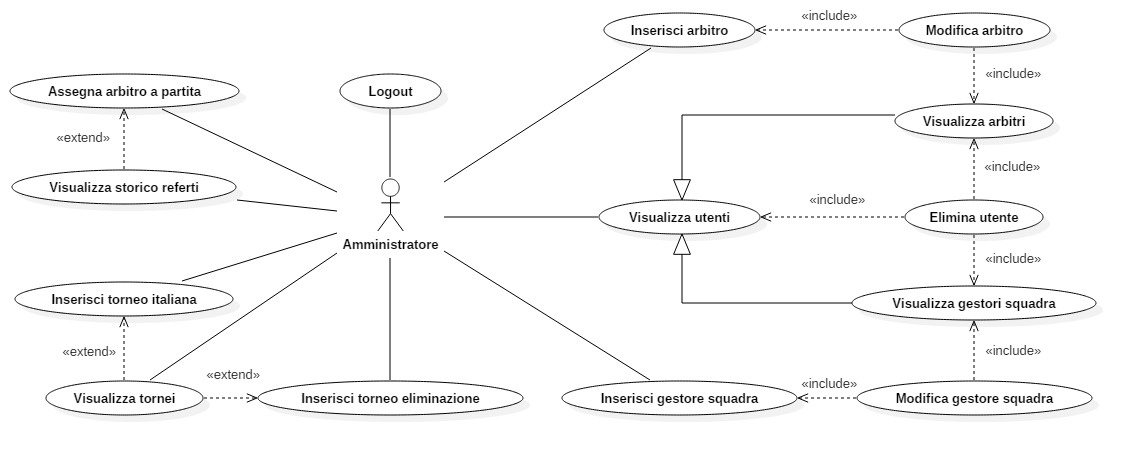
\includegraphics[width=1\textwidth]
	{immagini/uc-amministratore}
	
	\caption{Casi d'uso dell'attore amministratore}
\end{figure}

%
% Caso d'uso: Logout
%
\subsection{Caso d'uso: Logout}

\subsubsection*{Descrizione}
Questa funzionalità permette all'amministratore di uscire dalla sua pagina e di iniziare a navigare come utente pubblico.
Il pulsante di Logout è presente in ogni pagina dell'applicazione web, in alto a destra.

\subsubsection*{Attori coinvolti}
Amministratore, partecipazione attiva dell'attore verso il caso d'uso medesimo.

\subsubsection*{Pre-condizioni}
È richiesto l'accesso al sistema tramite la funzionalità di login.

\subsubsection*{Post-condizioni}
Termina la sessione di accesso al sistema in qualità di amministratore.

\subsubsection*{Flusso principale}

\begin{enumerate}
	
	\item
	L'amministratore seleziona nella pagina in cui si trova il pulsante di Logout;
	
	\item
	Il sistema scollega l'amministratore dalle pagine a lui riservate;
	
	\item
	Il sistema redireziona l'amministratore nella schermata di login e da quel momento può navigare come utente pubblico.
	
\end{enumerate}

\subsubsection*{Flussi alternativi}
Nel caso di operazione non riuscita si notifica all'amministratore il tipo di errore che si è verificato.

\subsection*{Diagramma delle attività}
Il diagramma delle attività per il caso d'uso ``Logout'' è illustrato nella figura \vref{ad-logout}.


%
% Caso d'uso: Inserisci arbitro
%
\subsection{Caso d'uso: Inserisci arbitro}
\label{uc-inserisci-arbitro}

\subsubsection*{Descrizione}
Questa funzionalità permette all'amministratore di creare un nuovo utente di tipo arbitro.

\subsubsection*{Attori coinvolti}
Amministratore, partecipazione attiva dell'attore verso il caso d'uso medesimo.
L'amministratore interagisce direttamente con il sistema compilando i campi richiesti.

Arbitro, partecipazione non attiva in quanto si procede solo alla creazione di tale attore.

\subsubsection*{Pre-condizioni}
È richiesto l'accesso al sistema come amministratore, tramite la funzionalità di login, in quanto solo lui ha il privilegio di poter inserire un arbitro.

\subsubsection*{Post-condizioni}
Viene aggiornato lo stato sul database con l'inserimento di un nuovo arbitro. L'arbitro è associato all'amministratore.

\subsubsection*{Flusso principale}

\begin{enumerate}
	
	\item
	L'amministratore seleziona la voce ``Nuovo Arbitro'' nella propria home page oppure seleziona la voce ``Inserisci Nuovo Arbitro''nella pagina di visualizzazione degli utenti;
	
	\item
	L'amministratore inserisce per l'arbitro i seguenti dati: nome, cognome, email, password, indirizzo, telefono, data di nascita, nazionalità, foto e carriera;
	
	\item
	L'amministratore invia la richiesta di creazione del nuovo utente al sistema;
	
	\item
	In caso di email già presente nel database viene notificato con un messaggio l'indisponibilità della email inserita invitando l'amministratore ad inserire una nuova mail;
	
	\item
	Se tutti i dati sono stati inseriti correttamente, il sistema inserisce l'arbitro nel database;
	
	\item
	Il sistema visualizza i dati dell'arbitro appena inserito dando la possibilità all'amministratore di modificare i dati.
	
\end{enumerate}

\subsubsection*{Flussi alternativi}
Nel caso di inserimento errato dei dati da parte dell'amministratore o di operazione non riuscita, si notifica all'amministratore il tipo di errore che si è verificato.


%
% Caso d'uso: Modifica arbitro
%
\subsection{Caso d'uso: Modifica arbitro}

\subsubsection*{Descrizione}
Questa funzionalità permette all'amministratore di modificare i dati di un arbitro presente nel database.

\subsubsection*{Attori coinvolti}
Amministratore, partecipazione attiva dell'attore verso il caso d'uso medesimo.
L'amministratore interagisce direttamente con il sistema modificando alcuni dei campi richiesti.

Arbitro, partecipazione non attiva in quanto si procede solo alla modifica di tale attore.

\subsubsection*{Pre-condizioni}
È richiesto l'accesso al sistema come amministratore, tramite la funzionalità di login, in quanto solo lui ha il privilegio di poter modificare un arbitro.

\subsubsection*{Post-condizioni}
Viene aggiornato lo stato sul database con la modifica di un arbitro.

\subsubsection*{Flusso principale}

\begin{enumerate}
	
	\item
	L'amministratore seleziona la voce ``Utenti'' nella pagina in cui si trova;
	
	\item
	L'amministratore seleziona la voce ``Arbitro'' per visualizzare gli utenti di tipo arbitro;
	
	\item
	L'amministratore seleziona la voce ``Modifica'', per l'arbitro che desidera modificare, nella lista degli arbitri;
	
	\item
	L'amministratore può modificare per l'arbitro i seguenti dati: nome, cognome, email, password, indirizzo, telefono, data di nascita, nazionalità, foto e carriera;
	
	\item
	L'amministratore invia la richiesta di modifica dell'arbitro al sistema;
	
	\item
	In caso di modifica dell'email con l'inserimento di una email già presente nel database, viene notificato, con un messaggio, l'indisponibilità della email inserita invitando l'amministratore ad inserire una nuova mail;
	
	\item
	Se tutti i dati sono stati inseriti correttamente, il sistema modifica l'arbitro nel database;
	
	\item
	Il sistema visualizza i dati dell'arbitro appena modificato dando la possibilità all'amministratore di effettuare ulteriori modifiche.
	
\end{enumerate}

\subsubsection*{Flussi alternativi}
Nel caso di operazione non riuscita, si notifica all'amministratore il tipo di errore che si è verificato.

\subsubsection*{Punti di inclusione}
Si può accedere a questo caso d'uso quando si effettua l'inserimento di un nuovo arbitro, vedi caso d'uso \vref{uc-inserisci-arbitro}, oppure quando si visualizza la lista di gli arbitri creati dall'amministratore, vedi caso d'uso \vref{uc-visualizza-arbitri}.


%
% Caso d'uso: Visualizza arbitri
%
\subsection{Caso d'uso: Visualizza arbitri}
\label{uc-visualizza-arbitri}

\subsubsection*{Descrizione}
Questa funzionalità permette di visualizzare la lista di tutti gli arbitri creati dall'amministratore.

\subsubsection*{Attori coinvolti}
Amministratore, partecipazione attiva dell'attore verso il caso d'uso medesimo.

\subsubsection*{Pre-condizioni}
È richiesto l'accesso al sistema come amministratore, tramite la funzionalità di login, in quanto solo lui ha il privilegio di poter visualizzare i propri arbitri.

\subsubsection*{Post-condizioni}
Nessuna post-condizione in quanto la visualizzazione degli arbitri non contribuisce a cambiare lo stato del sistema.

\subsubsection*{Flusso principale}

\begin{enumerate}
	
	\item
	L'amministratore seleziona la voce ``Utenti'' nella pagina in cui si trova;
	
	\item
	L'amministratore selezione la voce ``Arbitro'' nella pagina utenti;
	
	\item
	Il sistema visualizza tutti gli arbitri in ordine alfabetico mostrandone: id, cognome, nome, email, indirizzo e telefono. Il sistema, inoltre, visualizza per ogni utente un pulsante per eliminare l'utente e un pulsante per modificare l'utente.
	
\end{enumerate}

\subsubsection*{Flussi alternativi}
Nel caso di operazione non riuscita, si notifica all'amministratore il tipo di errore che si è verificato.


%
% Caso d'uso: Visualizza utenti
%
\subsection{Caso d'uso: Visualizza utenti}
\label{uc-visualizza-utenti}

\subsubsection*{Descrizione}
Questa funzionalità permette di visualizzare la lista di tutti gli utenti creati dall'amministratore.

\subsubsection*{Attori coinvolti}
Amministratore, partecipazione attiva dell'attore verso il caso d'uso medesimo.

\subsubsection*{Pre-condizioni}
È richiesto l'accesso al sistema come amministratore, tramite la funzionalità di login, in quanto solo lui ha il privilegio di poter visualizzare i propri utenti.

\subsubsection*{Post-condizioni}
Nessuna post-condizione in quanto la visualizzazione degli utenti non contribuisce a cambiare lo stato del sistema.

\subsubsection*{Flusso principale}

\begin{enumerate}
	
	\item
	L'amministratore seleziona la voce ``Utenti'' nella pagina in cui si trova;
	
	\item
	Il sistema visualizza tutti gli utenti in ordine alfabetico mostrandone: id, cognome, nome, email, indirizzo e telefono. Il sistema, inoltre, visualizza per ogni utente un pulsante per eliminare l'utente.
	
\end{enumerate}

\subsubsection*{Flussi alternativi}
Nel caso di operazione non riuscita, si notifica all'amministratore il tipo di errore che si è verificato.

\subsubsection*{Punti di specializzazione}
Questo caso d'uso si può specializzare in Visualizza Arbitri, vedi caso d'uso \vref{uc-visualizza-arbitri}, oppure Visualizza gestori squadra, vedi caso d'uso \vref{uc-visualizza-gestori-squadra}.


%
% Caso d'uso: Visualizza gestori squadra
%
\subsection{Caso d'uso: Visualizza gestori squadra}
\label{uc-visualizza-gestori-squadra}

\subsubsection*{Descrizione}
Questa funzionalità permette di visualizzare la lista di tutti i gestori di squadra creati dall'amministratore.

\subsubsection*{Attori coinvolti}
Amministratore, partecipazione attiva dell'attore verso il caso d'uso medesimo.

\subsubsection*{Pre-condizioni}
È richiesto l'accesso al sistema come amministratore, tramite la funzionalità di login, in quanto solo lui ha il privilegio di poter visualizzare i propri gestori di squadra.

\subsubsection*{Post-condizioni}
Nessuna post-condizione in quanto la visualizzazione dei gestori di squadra non contribuisce a cambiare lo stato del sistema.

\subsubsection*{Flusso principale}

\begin{enumerate}
	
	\item
	L'amministratore seleziona la voce ``Utenti'' nella pagina in cui si trova;
	
	\item
	L'amministratore selezione la voce ``Gestore'' nella pagina utenti;
	
	\item
	Il sistema visualizza tutti gli gestore di squadra in ordine alfabetico mostrandone: id, cognome, nome, email, indirizzo e telefono. Il sistema, inoltre, visualizza per ogni utente un pulsante per eliminare l'utente e un pulsante per modificare l'utente.
	
\end{enumerate}

\subsubsection*{Flussi alternativi}
Nel caso di operazione non riuscita, si notifica all'amministratore il tipo di errore che si è verificato.


%
% Caso d'uso: Inserisci gestore squadra
%
\subsection{Caso d'uso: Inserisci gestore squadra}
\label{uc-inserisci-gestore-squadra}

\subsubsection*{Descrizione}
Questa funzionalità permette all'amministratore di creare un nuovo utente di tipo gestore squadra.

\subsubsection*{Attori coinvolti}
Amministratore, partecipazione attiva dell'attore verso il caso d'uso medesimo.
L'amministratore interagisce direttamente con il sistema compilando i campi richiesti.

Gestore squadra, partecipazione non attiva in quanto si procede solo alla creazione di tale attore.

\subsubsection*{Pre-condizioni}
È richiesto l'accesso al sistema come amministratore, tramite la funzionalità di login, in quanto solo lui ha il privilegio di poter inserire un gestore di una squadra.

\subsubsection*{Post-condizioni}
Viene aggiornato lo stato sul database con l'inserimento di un nuovo gestore di squadra. Il gestore di squadra è associato all'amministratore.

\subsubsection*{Flusso principale}

\begin{enumerate}
	
	\item
	L'amministratore seleziona la voce ``Nuovo Gestore Squadra'' nella propria home page oppure seleziona la voce ``Inserisci Nuovo Gestore Squadra''nella pagina di visualizzazione degli utenti;
	
	\item
	L'amministratore inserisce per il gestore squadra i seguenti dati: nome, cognome, email, password, indirizzo, telefono e nome della squadra che andrà a gestire;
	
	\item
	L'amministratore invia la richiesta di creazione del nuovo utente al sistema;
	
	\item
	In caso di email già presente nel database viene notificato con un messaggio l'indisponibilità della email inserita invitando l'amministratore ad inserire una nuova mail;
	
	\item
	Se tutti i dati sono stati inseriti correttamente, il sistema inserisce nel database il gestore della squadra e una nuova squadra associato ad esso;
	
	\item
	Il sistema visualizza i dati del gestore appena inserito dando la possibilità all'amministratore di modificare i dati.
	
\end{enumerate}

\subsubsection*{Flussi alternativi}
Nel caso di inserimento errato dei dati da parte dell'amministratore o di operazione non riuscita, si notifica all'amministratore il tipo di errore che si è verificato.


%
% Caso d'uso: Modifica gestore squadra
%
\subsection{Caso d'uso: Modifica gestore squadra}

\subsubsection*{Descrizione}
Questa funzionalità permette all'amministratore di modificare i dati di un gestore squadra presente nel database.

\subsubsection*{Attori coinvolti}
Amministratore, partecipazione attiva dell'attore verso il caso d'uso medesimo.
L'amministratore interagisce direttamente con il sistema modificando alcuni dei campi richiesti.

Gestore squadra, partecipazione non attiva in quanto si procede solo alla modifica di tale attore.

\subsubsection*{Pre-condizioni}
È richiesto l'accesso al sistema come amministratore, tramite la funzionalità di login, in quanto solo lui ha il privilegio di poter modificare un gestore di una squadra.

\subsubsection*{Post-condizioni}
Viene aggiornato lo stato sul database con la modifica di un  gestore di una squadra.

\subsubsection*{Flusso principale}

\begin{enumerate}
	
	\item
	L'amministratore seleziona la voce ``Utenti'' nella pagina in cui si trova;
	
	\item
	L'amministratore seleziona la voce ``Gestore'' per visualizzare gli utenti di tipo gestore squadra;
	
	\item
	L'amministratore seleziona la voce ``Modifica'', per il gestore squadra che desidera modificare, nella lista degli arbitri;
	
	\item
	L'amministratore può modificare per l'arbitro i seguenti dati: nome, cognome, email, password, indirizzo, telefono e squadra;
	
	\item
	L'amministratore invia la richiesta di modifica dell'arbitro al sistema;
	
	\item
	In caso di modifica dell'email con l'inserimento di una email già presente nel database, viene notificato, con un messaggio, l'indisponibilità della email inserita invitando l'amministratore ad inserire una nuova mail;
	
	\item
	Se tutti i dati sono stati inseriti correttamente, il sistema modifica il gestore squadra nel database;
	
	\item
	Il sistema visualizza i dati del gestore squadra appena modificato dando la possibilità all'amministratore di effettuare ulteriori modifiche.
	
\end{enumerate}

\subsubsection*{Flussi alternativi}
Nel caso di operazione non riuscita, si notifica all'amministratore il tipo di errore che si è verificato.

\subsubsection*{Punti di inclusione}
Si può accedere a questo caso d'uso quando si effettua l'inserimento di un nuovo gestore squadra, vedi caso d'uso \vref{uc-inserisci-gestore-squadra}, oppure quando si visualizza la lista di tutti i gestori squadra creati dall'amministratore, vedi caso d'uso \vref{uc-visualizza-gestori-squadra}.


%
% Caso d'uso: Elimina utente
%
\subsection{Caso d'uso: Elimina utente}

\subsubsection*{Descrizione}
Questa funzionalità permette all'amministratore di eliminare un utente registrato e, conseguentemente, di invalidare l'accesso delle credenziali dell'utente eliminato all'applicazione web.

\subsubsection*{Attori coinvolti}
Amministratore, partecipazione attiva dell'attore verso il caso d'uso medesimo.
L'amministratore interagisce direttamente con il sistema eliminando l'utente selezionato.

\subsubsection*{Pre-condizioni}
È richiesto l'accesso al sistema come amministratore, tramite la funzionalità di login, in quanto solo lui ha il privilegio di poter eliminare i propri utenti.

\subsubsection*{Post-condizioni}
Viene aggiornato lo stato sul database con l'eliminazione dell'utente selezionato.

\subsubsection*{Flusso principale}

\begin{enumerate}
	
	\item
	L'amministratore seleziona la voce ``Elimina'', per l'utente che desidera eliminare, nella lista degli utenti;
	
	\item
	Il sistema chiede la conferma di esecuzione dell'operazione;
	
	\item
	Se l'amministratore conferma l'operazione l'utente viene eliminato altrimenti l'operazione viene annullata.
	
\end{enumerate}

\subsubsection*{Flussi alternativi}
Nel caso di operazione non riuscita, si notifica all'amministratore il tipo di errore che si è verificato.

\subsubsection*{Punti di inclusione}
Si può accedere a questo caso d'uso quando si effettua la visualizzazione di tutti gli utenti, vedi caso d'uso \vref{uc-visualizza-utenti}, quando si visualizza la lista di tutti gli arbitri creati dall'amministratore, vedi caso d'uso \vref{uc-visualizza-arbitri}, quando si visualizza la lista di tutti i gestori squadra creati dall'amministratore, vedi caso d'uso \vref{uc-visualizza-gestori-squadra}.


%
% Caso d'uso: Inserisci torneo eliminazione
%
\subsection{Caso d'uso: Inserisci torneo eliminazione}

\subsubsection*{Descrizione}
Questa funzionalità permette all'amministratore di creare un nuovo torneo ad eliminazione diretta.

\subsubsection*{Attori coinvolti}
Amministratore, partecipazione attiva dell'attore verso il caso d'uso medesimo.
L'amministratore interagisce direttamente con il sistema compilando i campi richiesti.

\subsubsection*{Pre-condizioni}
È richiesto l'accesso al sistema come amministratore, tramite la funzionalità di login, in quanto solo lui ha il privilegio di poter creare un torneo ad eliminazione.

\subsubsection*{Post-condizioni}
Viene aggiornato lo stato sul database con l'inserimento di un nuovo torneo ad eliminazione.

\subsubsection*{Flusso principale}

\begin{enumerate}
	
	\item
	L'amministratore seleziona la voce ``Nuovo Torneo Eliminazione'' nella propria home page o nella pagina di visualizzazione dei tornei;
	
	\item
	Il sistema restituisce la pagina web dove l'amministratore inserirà: il nome del torneo, il numero di squadre partecipanti e una descrizione relativa al torneo;
	
	\item
	L'amministratore prosegue con la creazione cliccando sul pulsante ``Continua'';
	
	\item
	Il sistema controlla che tutti i dati siano stati inseriti correttamente e visualizza la lista delle squadre complete presenti sul sistema (una squadra è completa quando il gestore di squadra ha compilato tutti i campi relativi alla propria squadra altrimenti la squadra non può partecipare ai tornei).
	
	\item
	L'amministratore seleziona le squadre da iscrivere al torneo;
	
	\item
	Il sistema controlla che sia stato inserito il giusto numero di squadre;
	
	\item
	Il sistema chiede la conferma all'amministratore e, in caso affermativo, il sistema crea il torneo;
	
	\item
	Il sistema notifica il successo dell'operazione all'amministratore visualizzando il tabellone degli incontri.
	
\end{enumerate}

\subsubsection*{Flussi alternativi}
Nel caso di inserimento errato dei dati da parte dell'amministratore o di operazione non riuscita, si notifica all'amministratore il tipo di errore che si è verificato.

\subsubsection*{Punti di estensione}
Si può accedere a questo caso d'uso quando si effettua la visualizzazione della lista di tutti i tornei creati dall'amministratore, vedi caso d'uso \vref{uc-visualizza-tornei}, ma si tratta di un accesso opzionale.


%
% Caso d'uso: Visualizza tornei
%
\subsection{Caso d'uso: Visualizza tornei}
\label{uc-visualizza-tornei}

\subsubsection*{Descrizione}
Questa funzionalità permette all'amministratore di vedere i tornei da lui creati e di monitorarne l'andamento.

\subsubsection*{Attori coinvolti}
Amministratore, partecipazione attiva dell'attore verso il caso d'uso medesimo.
L'amministratore richiede la visualizzazione delle pagine.

\subsubsection*{Pre-condizioni}
È richiesto l'accesso al sistema come amministratore, tramite la funzionalità di login.

\subsubsection*{Post-condizioni}
Nessuna post-condizione in quanto la visualizzazione dei tornei non contribuisce a cambiare lo stato del sistema.

\subsubsection*{Flusso principale}

\begin{enumerate}
	
	\item
	L'amministratore seleziona la voce ``Tornei'' nella pagina in cui si trova;
	
	\item
	Il sistema invia la pagina richiesta con la lista dei tornei creati dall'amministratore.
	
\end{enumerate}

\subsubsection*{Flussi alternativi}
Nel caso di operazione non riuscita, si notifica all'amministratore il tipo di errore che si è verificato.


%
% Caso d'uso: Inserisci torneo italiana
%
\subsection{Caso d'uso: Inserisci torneo italiana}

\subsubsection*{Descrizione}
Questa funzionalità permette all'amministratore di creare un nuovo torneo all'italiana.

\subsubsection*{Attori coinvolti}
Amministratore, partecipazione attiva dell'attore verso il caso d'uso medesimo.
L'amministratore interagisce direttamente con il sistema compilando i campi richiesti.

\subsubsection*{Pre-condizioni}
È richiesto l'accesso al sistema come amministratore, tramite la funzionalità di login, in quanto solo lui ha il privilegio di poter creare un torneo all'italiana.

\subsubsection*{Post-condizioni}
Viene aggiornato lo stato sul database con l'inserimento di un nuovo torneo all'italiana.

\subsubsection*{Flusso principale}

\begin{enumerate}
	
	\item
	L'amministratore seleziona la voce ``Nuovo Torneo Italiana'' nella propria home page o nella pagina di visualizzazione dei tornei;
	
	\item
	Il sistema restituisce la pagina web dove l'amministratore inserirà: il nome del torneo, il numero di squadre partecipanti e una descrizione relativa al torneo;
	
	\item
	L'amministratore prosegue con la creazione cliccando sul pulsante ``Continua'';
	
	\item
	Il sistema controlla che tutti i dati siano stati inseriti correttamente e visualizza la lista delle squadre complete presenti sul sistema (una squadra è completa quando il gestore di squadra ha compilato tutti i campi relativi alla propria squadra altrimenti la squadra non può partecipare ai tornei).
	
	\item
	L'amministratore seleziona le squadre da iscrivere al torneo;
	
	\item
	Il sistema controlla che sia stato inserito il giusto numero di squadre;
	
	\item
	Il sistema chiede la conferma all'amministratore e, in caso affermativo, il sistema crea il torneo;
	
	\item
	Il sistema notifica il successo dell'operazione all'amministratore visualizzando il tabellone delle varie giornate.
	
\end{enumerate}

\subsubsection*{Flussi alternativi}
Nel caso di inserimento errato dei dati da parte dell'amministratore o di operazione non riuscita, si notifica all'amministratore il tipo di errore che si è verificato.

\subsubsection*{Punti di estensione}
Si può accedere a questo caso d'uso quando si effettua la visualizzazione della lista di tutti i tornei creati dall'amministratore, vedi caso d'uso \vref{uc-visualizza-tornei}, ma si tratta di un accesso opzionale.

\subsection*{Diagramma delle attività}
Il diagramma delle attività per il caso d'uso ``Inserisci torneo all'italiana'' è illustrato nella figura \vref{ad-creazione-torneo-italiana}.


%
% Figura: diagramma delle attività relativo alla creazione del torneo all'italiana
%
\begin{figure}[h]
	\centering
	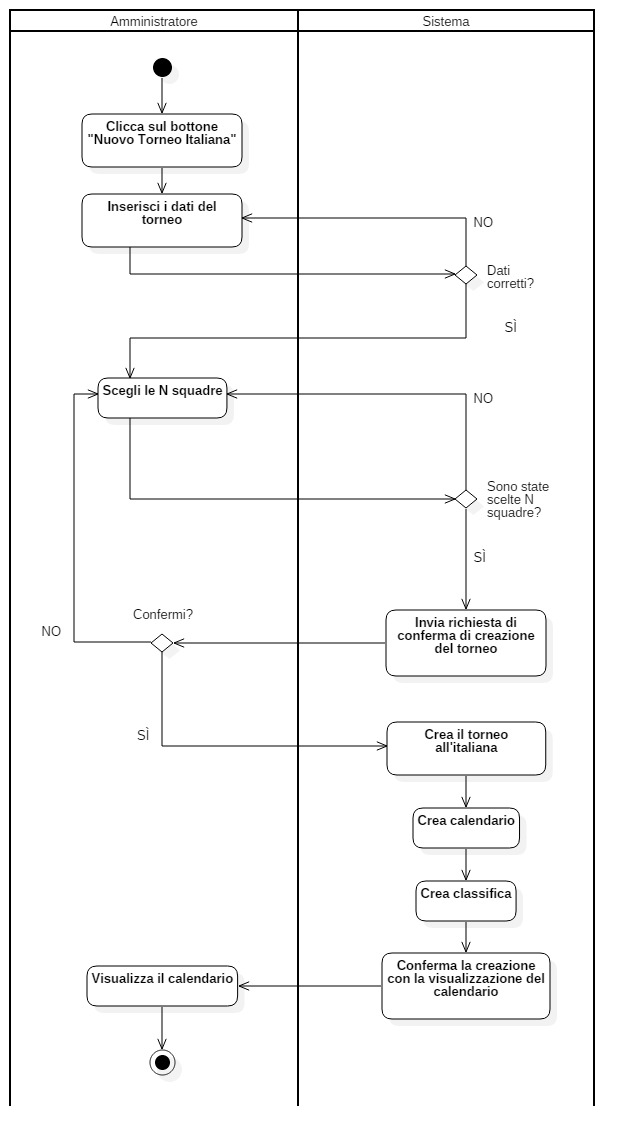
\includegraphics[width=0.8\textwidth]
	{immagini/ad-creazione-torneo-italiana}
	
	\caption{Diagramma delle attività della creazione di un torneo all'italiana}
	\label{ad-creazione-torneo-italiana}
\end{figure}


%
% Caso d'uso: Visualizza storico referti
%
\subsection{Caso d'uso: Visualizza storico referti}
\label{uc-visualizza-storico-referti}

\subsubsection*{Descrizione}
Questa funzionalità permette all'amministratore di vedere tutti i referti che l'amministratore ha assegnato ai rispettivi arbitri.

\subsubsection*{Attori coinvolti}
Amministratore, partecipazione attiva dell'attore verso il caso d'uso medesimo.
L'amministratore richiede la visualizzazione delle pagine.

\subsubsection*{Pre-condizioni}
È richiesto l'accesso al sistema come amministratore, tramite la funzionalità di login, in quanto solo lui ha il privilegio di poter visualizzare tale pagina.

\subsubsection*{Post-condizioni}
Nessuna post-condizione in quanto la visualizzazione dello storico dei referti non contribuisce a cambiare lo stato del sistema.

\subsubsection*{Flusso principale}

\begin{enumerate}
	
	\item
	L'amministratore seleziona la voce ``Referti'' nella pagina in cui si trova;
	
	\item
	Il sistema invia la pagina richiesta con la lista dei referti e dei rispettivi arbitri a cui sono stati assegnati dall'amministratore.
	
\end{enumerate}

\subsubsection*{Flussi alternativi}
Nel caso di operazione non riuscita, si notifica all'amministratore il tipo di errore che si è verificato.


%
% Caso d'uso: Assegna arbitro a partita
%
\subsection{Caso d'uso: Assegna arbitro a partita}

\subsubsection*{Descrizione}
Questa funzionalità permette all'amministratore di assegnare un arbitro ad una partita di un determinato torneo, associando all'arbitro un referto che dovrà essere compilato al termine della partita.

\subsubsection*{Attori coinvolti}
Amministratore, partecipazione attiva dell'attore verso il caso d'uso medesimo.
L'amministratore interagisce direttamente con il sistema compilando i campi richiesti.

Arbitro, partecipazione non attiva in quanto si procede solo all'assegnazione di un referto a tale attore.

\subsubsection*{Pre-condizioni}
È richiesto l'accesso al sistema come amministratore, tramite la funzionalità di login, in quanto solo lui ha il privilegio di poter assegnare un arbitro ad una partita di un torneo.

\subsubsection*{Post-condizioni}
Viene aggiornato lo stato sul database con l'inserimento di un nuovo referto e con l'associazione del referto appena creato con un arbitro presente nel database.

\subsubsection*{Flusso principale}

\begin{enumerate}
	
	\item
	L'amministratore seleziona la voce ``Assegna arbitro'' nella propria home page oppure seleziona la voce ``Assegna Arbitro a Partita'' nella pagina di visualizzazione dei referti;
	
	\item
	L'amministratore seleziona il torneo;
	
	\item
	L'amministratore seleziona la giornata/fase del torneo;
	
	\item
	Se per tale fase/giornata sono disponibili incontri non ancora assegnati, l'amministratore può selezionare la partita altrimenti il sistema visualizza un messaggio di indisponibilità delle partite;
	
	\item
	L'amministratore sceglie un arbitro ed inserisce per la partita: data, orario e luogo;
	
	\item
	L'amministratore preme il pulsante di ``Conferma assegnazione''.
	
	\item
	Il sistema chiede conferma all'amministratore dell'assegnazione dell'arbitro alla partita. Se l'amministratore acconsente il sistema elabora i dati, altrimenti non avviene alcuna operazione e permette all'amministratore di modificare i dati inseriti;
	
	\item
	Il sistema modifica lo stato del database aggiornando i dati della partita e inserendo un nuovo referto;
	
	\item
	Il sistema notifica l'amministratore l'esito positivo dell'operazione, visualizzando il referto appena inserito nello storico dei referti. 
	
\end{enumerate}

\subsubsection*{Flussi alternativi}
Nel caso di operazione non riuscita, si notifica all'amministratore il tipo di errore che si è verificato.

\subsubsection*{Punti di estensione}
Si può accedere a questo caso d'uso quando si effettua la visualizzazione della lista dello storico dei referti creati dall'amministratore, vedi caso d'uso \vref{uc-visualizza-storico-referti}, ma si tratta di un accesso opzionale.